% =============================================================================
%  Manuscript skeleton, Scientific Reports format (Article).
%  Storyline: ../audit/brief_2026-10-01/paper_storyline.md
%
%  Blue text in \note{...} is drafting guidance (content, numbers and their sources);
%  set \notesfalse below to hide it. Black text is draft prose.
%
%  Scientific Reports guide (checked 2026-11): main text <= ~4,500 words (excluding abstract,
%  Methods, references, legends), Methods unlimited, title <= 20 words, abstract <= 200 words,
%  unstructured, no references; <= 8 display items; ~60 references (not strict); legends
%  <= 350 words; Supplementary Information as one PDF; Data and Code availability statements;
%  LLM use documented in Methods.
%  Build: pdflatex main && bibtex main && pdflatex main && pdflatex main
% =============================================================================
\documentclass[11pt]{article}
\usepackage[a4paper,margin=2.5cm]{geometry}
\usepackage[T1]{fontenc}
\usepackage{lmodern}
\usepackage{amsmath,amssymb}
\usepackage{graphicx}
\usepackage{booktabs}
\usepackage{xcolor}
\usepackage[numbers,sort&compress]{natbib}
\usepackage{lineno}
\usepackage{setspace}
\usepackage{enumitem}
\usepackage[colorlinks=true,linkcolor=black,citecolor=black,urlcolor=blue]{hyperref}

\graphicspath{{../results/figures/}{../audit/brief_2026-10-01/pi_note/fig/}}

\newif\ifnotes \notestrue
\newcommand{\note}[1]{\ifnotes{\color{blue!70!black}\small\sffamily[#1]}\fi}
\newcommand{\um}{\,\textmu M/d}
\newcommand{\thci}{\theta_{\mathrm{crit}}^{\mathrm{int}}}
\newcommand{\dtr}{\Delta_{\mathrm{tr}}}

\linenumbers
\onehalfspacing

\title{The dose train is the identification experiment: sampling rules, limits on enzyme
capacity and dosing specifications in propionic acidaemia}
\author{Guido Putignano$^{1}$ \note{co-authors, affiliations, ORCID; corresponding author with
e-mail}}
\date{}

\begin{document}
\maketitle

\note{Title: 19 words (limit 20). Alternative, as one sentence of the main message: ``Infusion
schedules identify the enzyme half-life, not residual capacity, in severe propionic
acidaemia'' (13 words).}

% -----------------------------------------------------------------------------
\begin{abstract}
\noindent
An mRNA therapy for propionic acidaemia (PA) restores propionyl-CoA carboxylase (PCC) through
infusions, usually every two weeks; whether the interval can be lengthened is a central clinical
question. Its natural input, residual enzyme capacity, is not measured. Treating the dose train
as an identification experiment, we ask what routine blood sampling recovers. The infusions supply about 42 times
the excitation of the marker's own variation, and simple rules (sampling across the dose cycle,
never at the dose interval, and recording dosing and intake accurately) make capacity
identifiable to about $\pm20\%$ between 82\% and 627\% of normal, given a prior on the
non-enzymatic clearance. At 5\% of normal, typical of severe PA, no schedule or available
measurement reaches useful precision: with linear clearance the enzyme removes only 16\% of the
load, so it trades off against the other route, and direct activity assays lack a
calibrated scale. Dense sampling does identify change within one patient, as a difference, if
the marker's per-draw variability is below about 10\%. At baseline load the interval decision
reduces to a specification on PCC half-life and delivered dose, needing capacity only below a
crossing half-life. We give thresholds, late-infusion tolerances and a data specification.
\end{abstract}
\note{198 words (limit 200); recount after any edit. No references allowed.}

\noindent\textbf{Keywords:} practical identifiability; experiment design; propionic acidaemia;
mRNA therapy; dosing interval; enzyme replacement \note{up to 6}

% =============================================================================
\section*{Introduction}

Propionic acidaemia is an inborn error of metabolism caused by deficient propionyl-CoA
carboxylase (PCC). Residual PCC activity in patients' cultured fibroblasts is typically a few
per cent of control~\cite{pcc_residual_activity}. Patients manage a restricted protein intake and
remain at risk of acute metabolic decompensation, typically triggered by intercurrent
illness~\cite{pa_guidelines,pathophys_complications}.
mRNA-3927, an investigational mRNA therapy that makes the liver produce functional PCC, is given
as an intravenous infusion, every two weeks in four of the five phase 1/2 dose cohorts (every
three weeks in the first); interim results from that single-arm study reported fewer
decompensation events during treatment than before it, a reduction that was not statistically
significant (relative risk 0.30, 95\% CI 0.07--1.32)~\cite{trial_phase12}.
\note{Para 1, about 120 words. Disease, unmet need, the therapy, trial status. Cite
pa\_guidelines, genereviews\_pa, trial\_phase12, mrna\_moa, jiang2020dual.}

The clinical question this work starts from is the dosing interval: can infusions be spaced
further apart, for example every 15 or 21 days? The intuitive approach is to measure each
patient's residual capacity and dose accordingly. That capacity is not measured routinely, and
none of what the trial records (plasma markers, dated infusions, decompensation events, safety
monitoring) measures it directly.
\note{Para 2. Why the interval matters (burden of infusions, adherence, cost). Why residual
capacity looks like the natural decision variable.}

From the standpoint of systems identification the trial is already running an experiment: each
infusion is a known input that acts selectively on the enzyme channel, and every blood draw is
an output measured at some phase of the dose cycle, which the sampling schedule sets. The local
identification model is globally structurally identifiable from one patient whose marker moves
over a range of levels, though not at steady state; the question is practical identifiability,
with realistic noise, sampling and unknowns~\cite{profile_likelihood,nlme_identifiability}.
\note{Para 3. The control/identification framing, cite profile\_likelihood, curvature\_measures,
nlme\_identifiability, optimal\_input, design\_dose\_and\_times. Structural result: the
paper's proof (note\_structural\_identifiability).}

Here we ask four questions in turn. How should blood be sampled so that the dose train is
informative? Does that sampling identify residual capacity in severe PA? If not, what does the
record still identify? And what does the interval decision actually require? We answer them in a
metabolite-balance model with three hypotheses for the non-enzymatic clearance, compare the
conclusions against two published model structures, and end with a specification of the data
the trial should collect.
\note{Para 4. Contributions in one sentence each; roadmap of the Results.}

% =============================================================================
\section*{Results}

\subsection*{One balance, three hypotheses about one term}
The metabolite is produced by the dietary and endogenous load and removed through two exits:
the enzyme, with the patient's residual capacity $\theta$ plus the increment $\Delta(t)$
delivered by the infusions, and a non-enzymatic route $\alpha(m)$ (conjugation to carnitine and
renal loss). Our three models share this balance (Methods, Eq.~\eqref{eq:balance}) and differ
only in how $\alpha$ is written (in the parent model, through a carnitine state); the comparison
with published structures generates records from other balances. The \emph{parent model} derives $\alpha$ from the carnitine system:
it is the most realistic version, with a tipping point beyond which the patient decompensates,
and it defines the critical capacity used for dosing. The \emph{local identification model}
writes $\alpha=k_e m$, a straight line; it gives the best-conditioned joint fit of the two exits
(under the saturating variant the condition number is about 18 times larger), though not the
best precision on $\theta$ itself, which follows the enzyme's share of the load; it is used for
identifiability and design. The \emph{saturating variant} gives the route
a maximum speed and is used to test which conclusions depend on the straight line.
\note{Keep this section short in the main text (about 200 words); equations and constants in
Methods. Make explicit: one model, one disputed term, three hypotheses, each used for a stated
job (not a hierarchy of approximations). Sources: paper 02\_model, 03\_dynamic (remark that
the local model is not a reduction), pi\_note Setting.}

\subsection*{The dose train is the identification experiment}
\note{Message: the therapy does the identifying; how to sample. Figure~\ref{fig:sampling}.
Numbers (paper 06\_excitation, 07\_design, 08\_specification; normal capacity unless stated):
\begin{itemize}[nosep]
\item infusions supply about 42$\times$ the excitation of the marker band;
\item draws at the dose interval or a multiple see one phase: cost about 27$\times$, never
reach 0.20 (about 16$\times$ at 5\% of normal against the 14.5-day schedule);
\item fix: book every 14.5 days (half a day off): 0.16 over the full two-year record (51 visits;
not the 25-visit panel of Fig.~\ref{fig:sampling}b, which sweeps 89\% of one lap), ``monthly
precision at fortnightly density''; the schedule must sweep one lap of the dose cycle (lap rule);
\item monthly draws across cycles reach the target (0.17) given $k_e$ within a factor of 2.67 (the
paper's prior; without it $\theta$ is not identified) and the delivered increment known exactly;
then about a dozen visits suffice (target at 11). The increment must be known to a CV of 11.6\%;
at the published 14\% between-visit breath-test CV the target needs about 118 monthly draws;
\item the dosing record (date, dose, lot) is a regressor: carrying it is worth 7--16$\times$
with the $k_e$ prior;
\item intake as eaten, to better than about 10\%: accuracy matters, not variability;
\item antibiotic weeks recorded; no prior on $K_m$ needed; $K_m$ recovered to 6--7\% at every
capacity;
\item do not alter the dosing schedule for identification (about 13:1 against the patient);
first-hour post-infusion draws excluded from the steady-state fit.
\end{itemize}
Close with the scope: these rules reach the target only between 82\% and 627\% of normal.}

\begin{figure}[t]
\centering
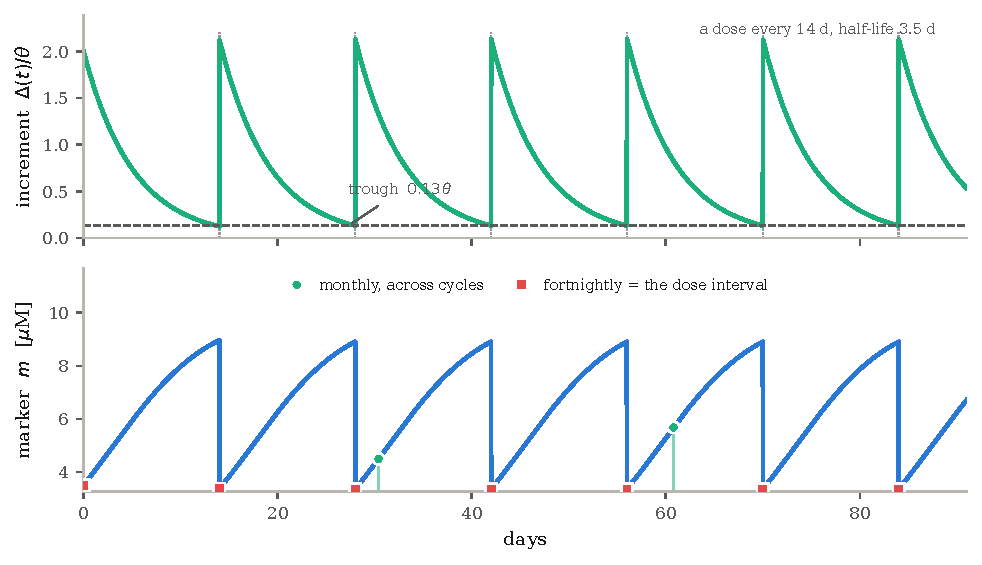
\includegraphics[width=0.48\linewidth]{fig_D0_dosetrain.pdf}\hfill
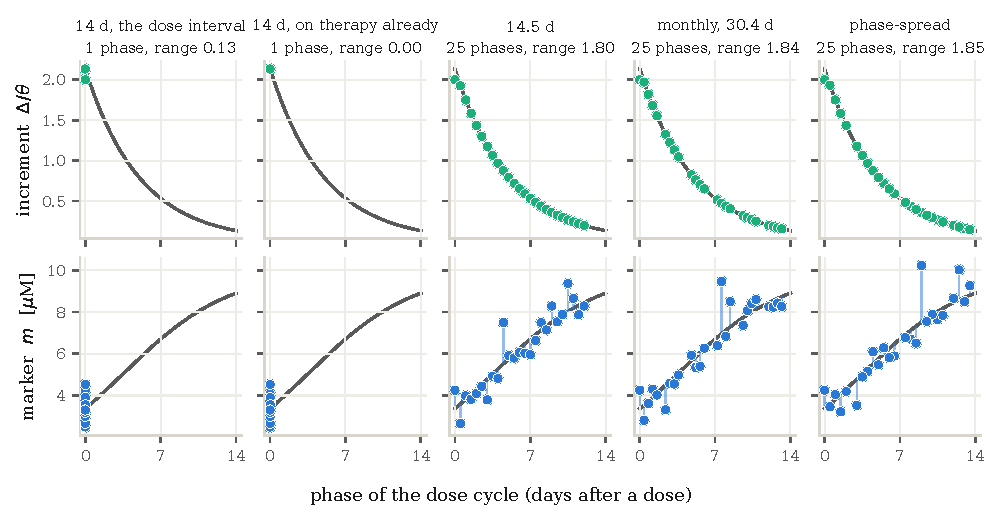
\includegraphics[width=0.48\linewidth]{fig_E1_phaseclock.pdf}
\caption{\label{fig:sampling}The dose train as the identification experiment. (a) The delivered
increment and the marker over successive infusions, with monthly draws across dose cycles and
draws at the dose interval, which all fall at one phase. (b) Where 25 draws of each schedule
land in the dose cycle: at the 14-day dose interval every draw falls at one phase, including when
sampling starts on therapy; a 14.5-day step reaches 25 of 28 phases (89\% of one lap; over a full
two-year record, 51 visits, it laps 1.8 times); monthly (30.4-day) and phase-spread schedules
cover the cycle. Both panels are at normal capacity. \note{Redraw as one two-panel figure at print size; legend $\le$350 words.}}
\end{figure}

\subsection*{The sampling rules hold across published model structures; the value of
\texorpdfstring{$\theta$}{theta} does not}
\note{Message: robustness of the design advice; structure-dependence of $\theta$; the cheap test.
Sources: paper A1\_supplementary (rem:structure\_relative), 11\_scope (structure dependence),
08\_specification Tier 1. Numbers:
\begin{itemize}[nosep]
\item records generated with Attarwala et al.~\cite{pkpd_translational} (algebraic $I_{\max}$)
and Gao et al.~\cite{dose_selection_poster} (turnover) structures;
\item schedule ranking unchanged; the two recommended designs agree to about 3\%;
\item $\hat\theta$ structure-relative: under the algebraic (Attarwala) structure $\theta$ is not
identifiable, and fitting our model to its records returns $\hat\theta$ 1.3--2.0$\times$ high at the
paper's dose and 4--20$\times$ at a trial-calibrated dose (with the paper's priors; several times
larger without), with a residual that can be under a fifth of $\sigma$; under the turnover (Gao)
structure $\theta$ is identifiable and the recommended schedules leave 2--3$\sigma$ of residual;
\item one draw 3 minutes after an infusion separates state-marker from algebraic-marker
structures by 16.3 standard deviations (9.7 at 15 min; 0.68 at 1 h); it rules out a family, not
every alternative.
\end{itemize}
Supplementary Table~S1. Wording: the design conclusions are robust to the published structures;
do not claim the models are ``similar''.}

\subsection*{Residual capacity is not practically identifiable in severe PA}
\note{Message: where the design works and why it fails at 5\%. Figure~\ref{fig:identifiability}.
Numbers (pi\_note Result 1; t1):
\begin{itemize}[nosep]
\item target $\operatorname{sd}(\ln\hat\theta)=0.20$ met only between 82\% and 627\% of normal;
best 0.123 at 212\%; 3.07 at 5\%; 14.75 at 1\%;
\item sampling 15$\times$ denser moves the lower edge from 82\% to 75\%: the limit is the
physiology, not the schedule;
\item profile likelihood: one-sided, $\theta$ below about 22\% of normal at 95\% (about 30\%
without the $k_e$ prior); no lower bound;
\item report bounds, not point estimates.
\end{itemize}}

\begin{figure}[t]
\centering
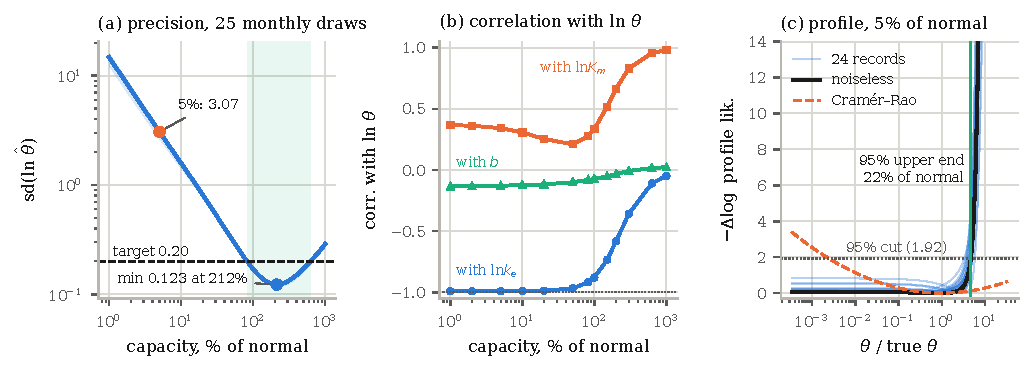
\includegraphics[width=\linewidth]{pi_t1.pdf}
\caption{\label{fig:identifiability}Practical identifiability of residual capacity. (a)
$\operatorname{sd}(\ln\hat\theta)$ of the monthly design against capacity; the target is met
only in the shaded band, 82--627\% of normal. (b) Correlation of $\ln\hat\theta$ with each other
unknown; below about 50\% of normal $\theta$ trades off almost perfectly against $k_e$. (c)
Profile likelihood at 5\% of normal: flat towards zero, a wall above about 22\% of normal; the
Cram\'er--Rao bowl misses both. \note{From pi\_note Fig.~1; expand legend.}}
\end{figure}

\subsection*{Why no available measurement closes the gap}
\note{Message: the paradox of indirect and direct measurement. Figures~\ref{fig:geometry} and
\ref{fig:routes}. Structure:
\begin{itemize}[nosep]
\item \emph{Indirect, through levels}: the record fixes the total cleared, not the split. The
``A + B'' arithmetic: at 5\% the enzyme removes 16\% and the other route 84\%; a 1\% error in
$k_e$ is a 5\% error in $\theta$; correlation $-0.99$, $k_e$ carries 98\% of the variance.
Worked example: $\theta$ anywhere from 0 to twice the truth needs $k_e$ to move only about 20\%
either way ($+19\%$ at $\theta=0$, $-19\%$ at twice the truth).
\item Geometry: each draw is a line $g(m_i)\theta+m_ik_e=\ldots$; similar levels give nearly
parallel lines (slopes $-0.0096$ to $-0.0073$), so the crossing is smeared. Spreading the draws
over untreated steady states at loads 0.45--3.2$\times$ the usual fans the lines and tightens the
fixed-$K_m$, prior-free $\operatorname{sd}(\ln\theta)$ about sevenfold (2.7 to 0.40, still twice the
target; 41\% of pairwise crossings within a factor of three), but only at loads far beyond the
parent model's fold.
\item Measuring $k_e$: IV $^{13}$C$_3$ tracer 0.45; both tracers 0.44; $k_e$ and the unrecorded
load exact 0.29.
\item \emph{Direct, through activity}: the ex vivo assay reaches 0.20 only with a cell-to-liver
scale nobody has measured; scale unknown 3.05; ratio to controls about 0.65. Breath test:
recovery uncalibrated.
\item No third way: in the model the enzyme acts only through the flow it carries.
\item Qualification: under the saturating variant the precision on $\theta$ is better
(0.29--0.92) but still misses without an unmeasured constant.
\end{itemize}}

\begin{figure}[t]
\centering
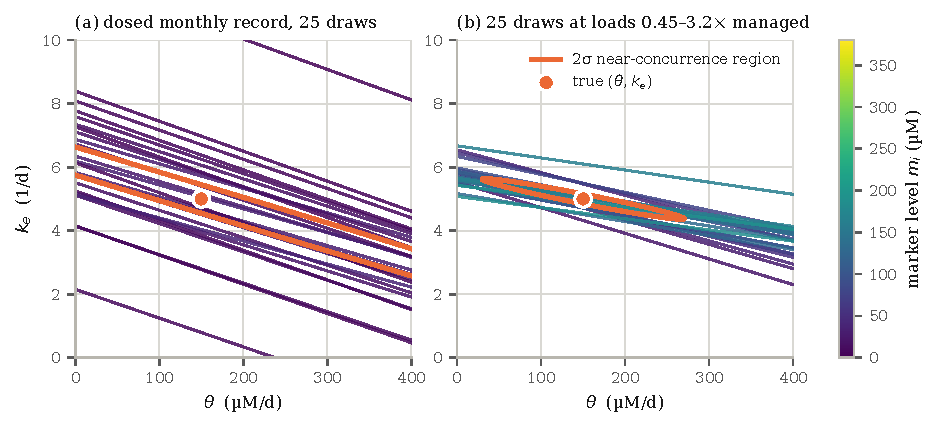
\includegraphics[width=0.86\linewidth]{pi_pencil.pdf}
\caption{\label{fig:geometry}Each steady-state draw as a line in the $(\theta,k_e)$ plane. (a)
The paper's monthly design: nearly parallel lines and a long region of near-concurrence. (b) An
imagined record at loads from 0.45 to 3.2 times the usual one, untreated: the lines fan out and
the region closes, at loads far beyond those the parent model tolerates.}
\end{figure}

\begin{figure}[t]
\centering
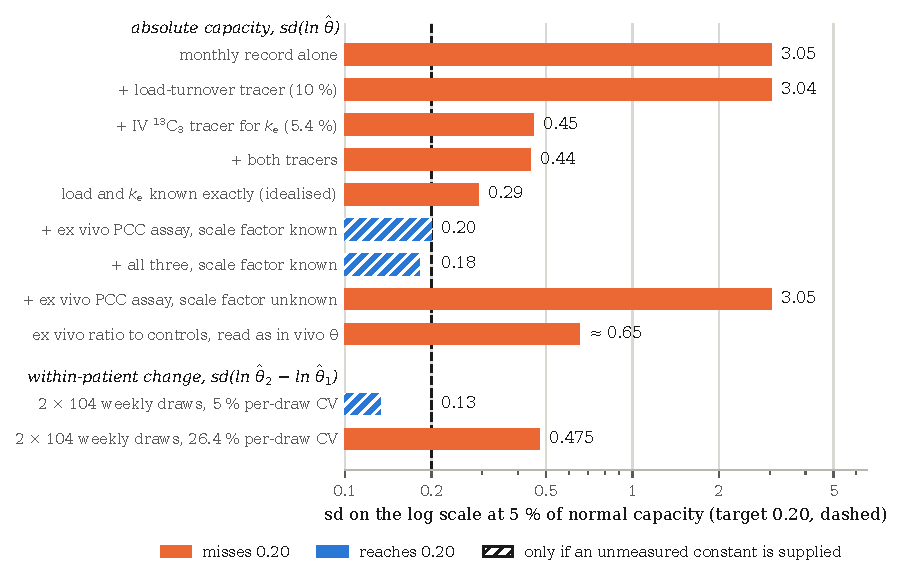
\includegraphics[width=0.86\linewidth]{pi_routes.pdf}
\caption{\label{fig:routes}Every route to $\theta$ at 5\% of normal. Upper group: absolute
capacity, $\operatorname{sd}(\ln\hat\theta)$. Lower group: the standard deviation of the change
between two windows, divided by the 150\um\ of a patient at 5\% of normal. The record-alone 3.05
differs from the 3.07 of Fig.~\ref{fig:identifiability} only in the noise model (here each draw
carries its own noise level, there one pooled level). Hatched bars reach 0.20 only if an
unmeasured quantity is supplied: a calibration (upper group) or a per-draw marker variability in
PA below about 10\% (lower group; bar drawn at 5\%).}
\end{figure}

\subsection*{Change within one patient is identifiable, as a difference}
\note{Message: what survives. Sources: pi\_note Result 3; t22, t24, t30, t42, t56 (simulated
pairs). Numbers:
\begin{itemize}[nosep]
\item the unknown constants shift both windows by the same amount and cancel in
$\hat\theta_2-\hat\theta_1$: two windows of 104 weekly draws give $\operatorname{sd}=20$\um\
(0.13 of the 150 of a 5\% patient); the difference test is calibrated (5\% false alarms) and
detects about 56\um\ with 80\% power (91\% for $+45\%$, 64\% for $-30\%$);
\item the ratio is not usable at 5\%: in about a quarter of simulated pairs an estimate falls to
zero; the log-ratio test raises false alarms a third of the time;
\item conditions: per-draw scatter $<$ about 10\% (C3 serial CV 26.4\%~\cite{thompson2012c3}
gives 71\um); $k_e$ drift of 0.06 in $\ln$ gives 42\um; a calibration shift of 1.5\% of the load
gives 30\um; gut-derived propionate is antibiotic-suppressible~\cite{metronidazole_pa}, so an
unrecorded antibiotic course through the second window fakes a rise of one to three times the
whole capacity (a linear-response estimate in the model). Clinical line: monitoring is feasible
if the marker proves stable; measuring its serial variability in PA is the first study to run.
\end{itemize}}

\subsection*{The dosing interval reduces to a specification on half-life and dose}
\note{Message: the decision does not need $\theta$. Figure~\ref{fig:margin},
Table~\ref{tab:spec}. Sources: pi\_note Result 4; t44, t52, t53, t54. Points:
\begin{itemize}[nosep]
\item trough condition: an interval keeps every patient maintainable if
$\dtr(\tau)>\thci$ (Methods, Eq.~\eqref{eq:trough}); $\thci=150.8$\um\ at the parent's
baseline load of 600\um;
\item crossings at the assumed dose: 2.62, 2.75, 3.55\,d (14, 15, 21 days); over the paper's
carnitine ranges 3.29--3.95\,d for 21 days; the critical capacity spans 110--232 over those
ranges (factor 2.1);
\item the paper's ceiling (enzyme never above normal) caps the dose below the assumed one: 21-day
crossing 4.47--5.80\,d;
\item likely hepatic half-life about 4.3\,d (plausibly 3--6), from mouse liver mitochondria
4.26\,d~\cite{kim2012} and the drug in mouse liver~\cite{pkpd_translational,jiang2020dual}; only
human value 3.6\,d in fibroblasts~\cite{chandler1985};
\item at 4.3\,d (if right; it rests on comparators): all intervals safe at the assumed dose
whatever the carnitine constants; at the capped dose 14 and 15 days stay safe (narrowly at the
least favourable constants) and 21 days needs, at the nominal constants, about 1.8\% of normal of
the patient's own capacity;
\item with the hepatic half-life log-normal about 4.3\,d (sd of $\ln$ 0.35--0.53) the probability
of clearing the nominal 21-day crossing is only 64--71\% (56--60\% at the least favourable
constants, 34--39\% at the capped dose);
\item the specification holds for the intrinsic threshold at baseline load; against the paper's
illness-amplitude threshold (994\um\ at $m_{\mathrm{tol}}=40$\,\textmu M) the 14-, 15- and 21-day
crossings at the assumed dose are about 5.0, 5.2 and 6.3\,d, so at 4.3\,d the booking again
depends on $\theta$;
\item where the half-life could be found: the sponsor's population model~\cite{dose_selection_poster},
which may hold a human protein-decay term but whose parameters are not public (a request to its
authors);
the dated on-therapy record ($\operatorname{sd}(\ln\lambda)=0.055$ after two years monthly; one
patient cannot place a value near a crossing, pooling 23--155 patients); a turnover study in
human hepatocytes;
\item estimating $\theta$ instead does not rescue the 21-day interval (margin sd about
95\um\ even with both tracers).
\end{itemize}}

\begin{figure}[t]
\centering
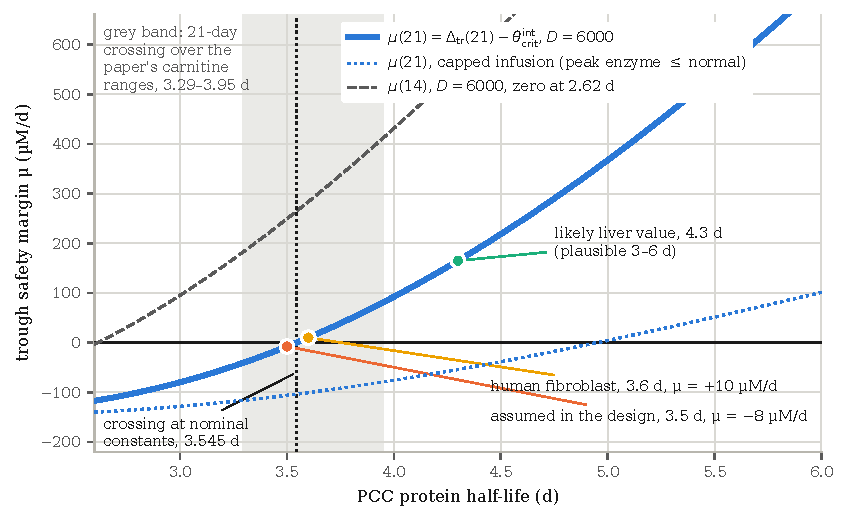
\includegraphics[width=0.74\linewidth]{pi_margin.pdf}
\caption{\label{fig:margin}Trough margin of a patient with no residual capacity against the PCC
protein half-life. Above zero an interval keeps every patient maintainable without knowing
$\theta$. Solid: 21 days at the assumed dose; dotted: 21 days at the dose capped by the ceiling;
dashed: 14 days. Grey band: the 21-day crossing over the paper's carnitine ranges. Dots: the
design's 3.5\,d, the fibroblast 3.6\,d and the likely hepatic 4.3\,d.}
\end{figure}

\begin{table}[t]
\centering\small
\caption{\label{tab:spec}The dosing specification: PCC half-life (days) above which an interval
keeps every patient maintainable at baseline load, whatever $\theta$. Ranges are over the corners
of the paper's carnitine-constant ranges.}
\begin{tabular}{@{}lcccc@{}}
\toprule
& \multicolumn{2}{c}{assumed dose, $D=6000$} & \multicolumn{2}{c}{capped at the ceiling} \\
\cmidrule(lr){2-3}\cmidrule(l){4-5}
interval & nominal & over the constants & nominal & over the constants \\
\midrule
14 days & $2.62$ & $2.41$--$2.95$ & $3.30$ & $2.98$--$3.87$ \\
15 days & $2.75$ & $2.54$--$3.10$ & $3.54$ & $3.19$--$4.15$ \\
21 days & $3.55$ & $3.29$--$3.95$ & $4.95$ & $4.47$--$5.80$ \\
\bottomrule
\end{tabular}
\end{table}

\subsection*{How late can an infusion be?}
\note{Message: tolerance to delays, alone and during illness. Figure~\ref{fig:tolerance};
Supplementary Table~S2 (delays by setting). Sources: pi\_note Result 5; t55. Numbers (booked
dose, nominal constants, 4.3\,d, $k=1$):
\begin{itemize}[nosep]
\item about $+10\%$ on the peak per day; doubling after 6.5--9 days (0--5\% of normal); skipped
infusion 3--5$\times$, with no lasting effect (first cycle after resumption about 7\% above);
\item illustrative illness (1.5$\times$ load for 14 days from the due day): about 2.5$\times$
even on time; 4--5$\times$ three days late and 15--21$\times$ a week late (no enzyme of their own to
2.5\% of normal; 3.7$\times$ and 10$\times$ at 5\%); at $k=1$ a one-day delay
does not raise the peak further;
\item least favourable settings (the paper's admissible dose $D=2672$, least favourable carnitine
corner, 3.5\,d half-life): doubling after about 2.5 days (about 4.3 days at the likely 4.3\,d); the trough condition is the
stricter test in 6 of 8 settings;
\item $k=10$: doubling delays shorter by under a day; peaks with a late infusion during illness
about 30\% higher (three days late 5--6$\times$, a week late 19--27$\times$); on-time illness peaks
little changed (2.5--2.8$\times$);
\item a late infusion is also a measurement of the half-life.
\end{itemize}}

\begin{figure}[t]
\centering
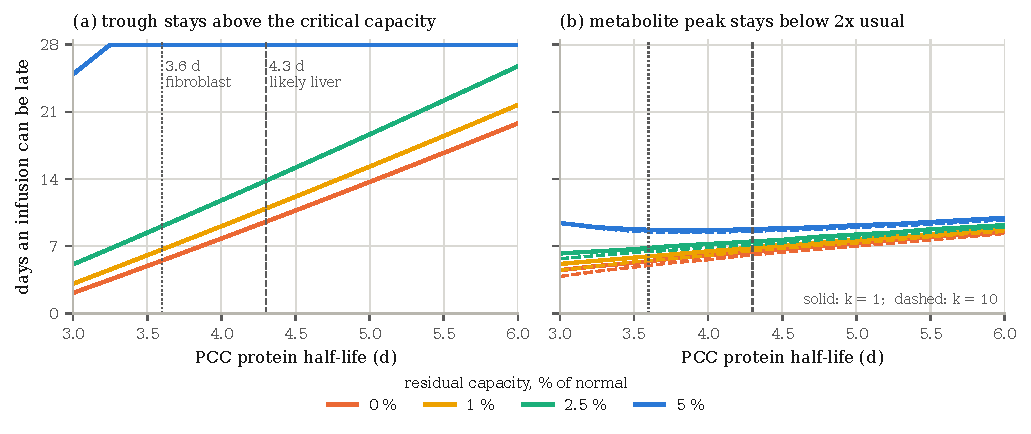
\includegraphics[width=\linewidth]{pi_tolerance.pdf}
\caption{\label{fig:tolerance}A late infusion in the parent model (half-life 4.3\,d, assumed
dose, nominal constants). (a) The metabolite of a patient with no enzyme of their own with the
infusion due at day 28 given on time, 3 or 7 days late, or skipped. (b) The highest level
reached, as a multiple of the usual peak, against days late (14 days late is a skipped
infusion); blue without illness, orange with the illustrative illness (1.5 times the baseline load
for 14 days from the day the infusion is due); solid, no enzyme of their own; dashed, 2.5\% of
normal; the illness curves stop where the metabolite passes the model's validity limit
($5.5\,M_i=1650$\,\textmu M).}
\end{figure}

% =============================================================================
\section*{Discussion}

\note{No subheadings. About 900 words. Paragraph plan:
\begin{enumerate}[nosep]
\item What the work shows, in one paragraph: the therapy is the experiment; good sampling makes
it informative; in severe PA capacity stays out of reach; the decision does not need it if the
half-life clears the crossing.
\item Model-informed specifications for the trial (Table~\ref{tab:data}): the
three tiers in order of dependency; the record; the interval; monitoring; safety (antibiotics,
on-time infusions during illness, stated as a model finding: on time the rise is about
2.5$\times$, three days late 4--5$\times$; whether to infuse during an illness is a clinical
decision; report bounds).
\item Relation to the literature: the sponsor's PK/PD and population
models~\cite{pkpd_translational,dose_selection_poster}; breath testing as a surrogate
endpoint~\cite{breath_test_mma}; identifiability practice in pharmacometrics.
\item Considerations and limitations: simulated records on illustrative constants; the local
model's 84\% non-enzymatic share is above literature estimates; the stable inter-crisis patient
only; the dosing specification uses the intrinsic threshold at baseline load (against the
paper's illness-amplitude threshold the crossings are about 5.0, 5.2 and 6.3\,d); the $k_e$ prior
behind the 82--627\% band has no published source; the within-patient result is from the local
model (0.088 relative to $\theta$ under the saturating variant, a Cram\'er--Rao value; not
computed under the parent); no propionyl-CoA state, so C3 and 2-methylcitrate are not
represented; $\hat\theta$ is relative to the assumed structure; the critical capacity rests on unmeasured carnitine constants (factor 2.1); the
``peak doubled'' yardstick and the illness are illustrative; $k$ assumed; not clinical
recommendations for an investigational drug.
\item Outlook: what would settle the open points (hepatic half-life, delivered increment, the
marker's serial CV in PA, a paired ex vivo/in vivo study); applying the method to the trial's
own dated record.
\end{enumerate}}

\begin{table}[t]
\centering\small
\caption{\label{tab:data}Data specification for the trial, in order of dependency.}
\begin{tabular}{@{}p{0.26\linewidth}p{0.68\linewidth}@{}}
\toprule
item & specification and purpose \\
\midrule
Tier 1: one post-infusion draw & one blood draw about 3 minutes after one infusion (within 15
minutes); rules out the published algebraic-marker structure, under which $\theta$ is not
identifiable at any design, but not every alternative \\
Tier 2: breath-test repeatability & two 1-$^{13}$C-propionate breath tests around one dose on
one day; coefficient of variation on the increment below about 12\%; the same-day
repeatability a pre/post measurement of the delivered increment needs \\
Tier 3: the record & draws spread across the dose cycle, never at the dose interval or a
multiple of it (monthly, or visits booked every 14.5 days over the whole record); dated infusions with dose and lot; intake as eaten, to better than about 10\%;
antibiotic weeks; no first-hour draw in the steady-state fit \\
For the interval & hepatic PCC half-life and delivered increment, against Table~\ref{tab:spec} \\
For monitoring & the marker's serial variability in PA (needs $<$ about 10\%); regimen and
antibiotic status fixed between comparison windows \\
\bottomrule
\end{tabular}
\note{Check every row against paper 08\_specification (tab:spec) and the PI note.}
\end{table}

% =============================================================================
\section*{Methods}

\subsection*{Model}
The metabolite level $m(t)$ (plasma 3-hydroxypropionate) obeys
\begin{equation}
\label{eq:balance}
\dot m = L(t) + L_0 - \bigl(\theta+\Delta(t)\bigr)\,g(m) - \alpha(m),
\qquad g(m)=\frac{m}{K_m+m},
\end{equation}
with recorded load $L(t)$, unrecorded load $L_0$, residual capacity $\theta$ (normal
3000\um), the increment delivered by the infusions
$\Delta(t)=D\sum_{k:\,t_k\le t} e^{-\lambda(t-t_k)}$ over past infusions at times $t_k$ ($D$ the
jump at each fortnightly dose) with $\lambda=\ln2/t_{1/2}$, and the non-enzymatic
clearance $\alpha(m)$. The three hypotheses are
\begin{gather}
\alpha_{\mathrm{parent}}(m)=\frac{R_0\,u}{u+\rho},\qquad
u=\frac{m}{K_c+m},\qquad\rho=\rho_0\Bigl(1+\frac{m}{M_i}\Bigr);\\
\alpha_{\mathrm{local}}(m)=k_e m;\qquad
\alpha_{\mathrm{sat}}(m)=\frac{V_e\,m}{K_e+m},
\end{gather}
\note{State the parent's two-state carnitine system and its quasi-steady reduction; constants
($K_m=100$\,\textmu M, $k_e=5$\,d$^{-1}$, $K_c=100$, $M_i=300$, $\rho_0=0.5$, $R_0$ derived so
that the route peaks at 500\um); saturating variant $V_e=400$\um, $K_e=300$\,\textmu M (its
maximal rate, not the local $k_e$); operating points (local: load 323\um, $\theta=3000$; parent:
baseline load 600\um); the tipping point and $\thci$; validity limit $m\approx5.5M_i$. Sources:
paper 02\_model, 03\_dynamic; src/common/params.py.}

\subsection*{Measurement and noise model}
\note{Plasma marker with 5\% assay CV; recorded load with 5\% error and 10\% day-to-day
variation; unrecorded load offset $b$ with prior 5\% of $L$; $k_e$ log-normal prior with sd 0.8;
draws excluded in the post-infusion settling window. Sources: core.py, paper 07\_design.}

\subsection*{Identifiability analysis}
\note{Fisher information and Cram\'er--Rao bounds on the log scale for
$(\ln\theta,\ln K_m,b,\ln k_e)$; profile likelihood; simulated fits (Monte Carlo) for
natural-scale and one-sided quantities, and wherever $\hat\theta$ can reach zero; 24 simulated
intake records. Cite profile\_likelihood, curvature\_measures, boundary\_lrt,
boundary\_bootstrap.}

\subsection*{Sampling design}
\note{Schedules compared (fortnightly at the dose interval, 14.5-day, monthly, two-monthly,
every two days); the lap rule $n\epsilon\ge T$; visits to reach the target; dose-calibration and
intake-accuracy sensitivity. Source: paper 06\_excitation, 07\_design.}

\subsection*{Comparison with published model structures}
\note{How records were generated with the Attarwala and Gao structures and analysed with ours;
what was compared (schedule ranking, recommended designs, $\hat\theta$); the 3-minute draw
separation. Source: paper A1\_supplementary, 11\_scope.}

\subsection*{Dosing interval: the trough condition}
For a dose train of interval $\tau$ delivering the same amount per day as the fortnightly
schedule, the increment at the trough is
\begin{equation}
\label{eq:trough}
\dtr(\tau)=D\,\frac{\tau}{14}\,\frac{e^{-\lambda\tau}}{1-e^{-\lambda\tau}},
\end{equation}
and a patient at baseline load stays maintainable through the cycle while
$\theta+\dtr(\tau)>\thci$, the parent model's intrinsic critical capacity (its fold at baseline
load). The interval keeps every patient maintainable at baseline load, whatever $\theta$, when
$\dtr(\tau)>\thci$ alone; against a critical capacity defined with an illness amplitude the
crossings are longer (about 5.0, 5.2 and 6.3\,d for 14, 15 and 21 days at the assumed dose).
\note{Intrinsic critical capacity (fold of the parent model at baseline load); the corners of
the paper's carnitine ranges with $R_0$ re-derived; the ceiling (peak enzyme no higher than
normal) applied at each interval; log-normal uncertainty on the hepatic half-life; half-life
identification from the dated on-therapy record (jitter, missed doses, a supply gap). Sources:
t44, t46, t52, t53, t54.}

\subsection*{Late infusions}
\note{Two-state parent model; eight on-time infusions, one late or skipped, then infusions every
14 days from it; peak window to 3 days after the late dose, during illness to the infusion after
it; doubling found by bisection to 0.025\,d; eight carnitine corners; $k=1$ and $k=10$; validity
limit. Source: t55.}

\subsection*{Within-patient change}
\note{Two windows of 104 draws over two years each; $k_e$, $b$ and $K_m$ shared; difference and
log-ratio tests; 400 simulated pairs per scenario. Sources: t22, t24, t30, t42, t56.}

\subsection*{Use of large language models}
\note{Required by the journal: document here which tools were used, their versions, for which
tasks (for example analysis code, verification of numbers, drafting and editing), and how the
authors verified the outputs. Write this section yourselves and keep it accurate.}

\subsection*{Software and reproducibility}
\note{Python (NumPy, SciPy), symbolic checks; repository with run scripts and outputs; every
number generated by a script.}

% =============================================================================
\section*{Data availability}
\note{All data are simulated; deposit the generated records and outputs (e.g.\ Zenodo, with
DOI).}

\section*{Code availability}
\note{Repository and archived release with DOI; licence.}

\section*{Author contributions}
\note{CRediT statement.}

\section*{Competing interests}
\note{Statement.}

\section*{Supplementary Information (outline)}
\note{\begin{itemize}[nosep]
\item S1: Model details, structural identifiability (paper note and supplement).
\item S2: Sampling design: full schedule comparison, visits, intake accuracy, dose calibration,
antibiotic weeks (paper Figs D1, E2, E3).
\item S3: Comparison with published structures (Table S1).
\item S4: Measurement routes in detail; saturating variant.
\item S5: Within-patient change: simulated pairs, drift, variability (t56, t24, t30, t42).
\item S6: Dosing specification over the carnitine constants; half-life from the record; the
ceiling.
\item S7: Late infusions by setting (Table S2), $k$ sensitivity, illness.
\item S8: Robustness and audit of the numbers (FIM against simulation).
\end{itemize}}

\bibliographystyle{unsrtnat}
\bibliography{../paper/refs,refs_extra}

\end{document}
